% ANUfinalexam.tex (Version 2.0)
% ===============================================================================
% Australian National University Final Exam LaTeX template.
% 2004; 2009, Timothy Kam, ANU School of Economics
% Licence type: Free as defined in the GNU General Public Licence: http://www.gnu.org/licenses/gpl.html

\documentclass[a4paper,10pt,leqno]{article}
\usepackage[fleqn]{mathtools}
\usepackage[labelformat=empty]{caption}
\usepackage{fancyhdr}
\usepackage{float}
\usepackage{tikz}
\usetikzlibrary{shapes}

% Insert your course information here %%%%%%%%%%%%%%%%%%%%%%%%%%%%%%%%%%

\newcommand{\institution}{UNIVERSITY OF THE PHILIPPINES DILIMAN}
\newcommand{\titlehd}{Database Systems}
\newcommand{\examtype}{Second Exam (Answer Key)}
\newcommand{\examdate}{March 15, 2014}
\newcommand{\examcode}{CS165}
\newcommand{\writetime}{THREE Hours}
\newcommand{\lastwords}{End of Exam}

%%%%%%%%%%%%%%%%%%%%%%%%%%%%%%%%%%%%%%%%%%%%%%%%%%%%

% ANU Exams Office mandated margins and footer style
\setlength{\topmargin}{0cm}
\setlength{\textheight}{9.25in}
\setlength{\oddsidemargin}{0.0in}
\setlength{\evensidemargin}{0.0in}
\setlength{\textwidth}{16cm}
\pagestyle{fancy}
\lhead{} 
\chead{} 
\rhead{} 
\lfoot{} 
\cfoot{\footnotesize{Page \thepage \ of \pageref{finalpage} -- \titlehd \ (\examcode)}} 
\rfoot{}

% DEPRECATED: ANU Exams Office mandated margins and footer style
%\setlength{\topmargin}{0cm}
%\setlength{\textheight}{9.25in}
%\setlength{\oddsidemargin}{0.0in}
%\setlength{\evensidemargin}{0.0in}
%\setlength{\textwidth}{16cm}
%\pagestyle{fancy}
%\lhead{} %left of the header
%\chead{} %center of the header
%\rhead{} %right of the header
%\lfoot{} %left of the footer
%\cfoot{} %center of the footer
%\rfoot{Page \ \thepage \ of \ \pageref{finalpage} \\
%       \texttt{\examcode}} %Print the page number in the right footer

\renewcommand{\headrulewidth}{0pt} %Do not print a rule below the header
\renewcommand{\footrulewidth}{0pt}

\begin{document}

% Title page

\begin{center}
%\vspace{5cm}
\large\textbf{\institution}
\end{center}
\vspace{1cm}

\begin{center}
\textit{ \examtype -- \examdate}
\end{center}
\vspace{1cm}

\begin{center}
\large\textbf{\titlehd}
\end{center}

\begin{center}
\large\textbf{\examcode}
\end{center}
\vspace{4cm}

\begin{center}
\textit{Writing Time:  \writetime}
\end{center}

% End title page

\newpage
\noindent{\textbf{Section 1: True or False [10 points]}\\\\}
\noindent Write {\textbf T} if the statement is true. If the statement is false, write {\textbf F}.

\vskip.10in
\noindent 1. {\textbf F} \\
\noindent 2. {\textbf T} \\
\noindent 3. {\textbf F} \\
\noindent 4. {\textbf T} \\
\noindent 5. {\textbf F} \\
\noindent 6. {\textbf T} \\
\noindent 7. {\textbf F} \\
\noindent 8. {\textbf F} \\
\noindent 9. {\textbf T} \\
\noindent 10. {\textbf T}

\vskip.35in
\noindent{\textbf{Section 2: Functional Dependencies [10 points]}}

\vskip.10in
\noindent {\textit i.} Functional dependencies:

\begin{itemize}
\item $custid \rightarrow custname$
\item $custid \rightarrow address$
\item $address \rightarrow zipcode$
\item $custid \rightarrow email$
\item $ordernum \rightarrow orderdate$
\item $itemnum \rightarrow itemname$
\item $supplier \rightarrow suppliertin$
\item $suppliertin \rightarrow suppliertaxstatus$
\end{itemize}

\noindent {\textit ii.} Decomposition:

\begin{itemize}
\item $Customers(custid, custname, address, zipcode, telephone, email)$
\item $Orders(custid, ordernum, orderdate)$
\item $OrderItems(ordernum, itemnum, quantity)$
\item $Items(itemnum, itemname, sellingprice)$
\item $ItemsSoldBy(itemnum, supplier)$
\item $Suppliers(supplier, suppliertaxstatus, suppliertin)$
\end{itemize}

\newpage

\noindent{\textbf{Section 3: Concurrency [10 points]}}

\vskip.10in
\noindent Precedence for A:

\begin{itemize}
\item $T_2 < T_1 (r_2 < w_1)$
\item $T_3 < T_1 (r_3 < w_1)$
\end{itemize}

\vskip.10in
\noindent Precedence for B:

\begin{itemize}
\item $T_1 < T_2 (r_1 < w_2)$
\item $T_4 < T_2 (r_4 < w_2)$
\end{itemize}

\vskip.10in
\noindent There exists a cycle in the schedule, thus it is not conflict-serializable.

\vskip.35in
\noindent{\textbf{Section 4: Index Structures [10 points]}}

\vskip.10in
\noindent After deleting 7:

\begin{center}
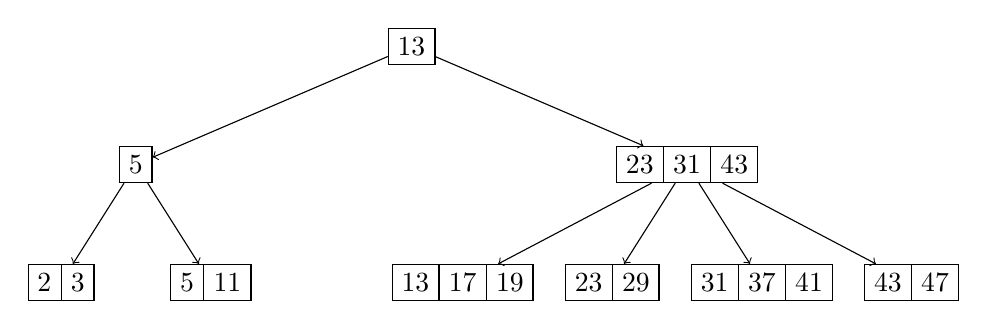
\begin{tikzpicture}
\tikzstyle{bplus}=[
  rectangle split,
  rectangle split horizontal,
  rectangle split ignore empty parts,
  draw ]
\tikzstyle{every node}=[bplus]
\tikzstyle{level 1}=[sibling distance=70mm]
\tikzstyle{level 2}=[sibling distance=19mm]
\node {13} [->]
  child {node {5}
    child {node {2 \nodepart{two} 3}}
    child {node {5 \nodepart{two} 11}}
  }
    child {node {23 \nodepart{two} 31 \nodepart{three} 43}
    child {node {13 \nodepart{two} 17 \nodepart{three} 19}}
    child {node {23 \nodepart{two} 29}}
    child {node {31 \nodepart{two} 37 \nodepart{three} 41}}
    child {node {43 \nodepart{two} 47}}
  }
;
\end{tikzpicture}
\end{center}

\vskip.10in
\noindent After deleting 17:

\begin{center}
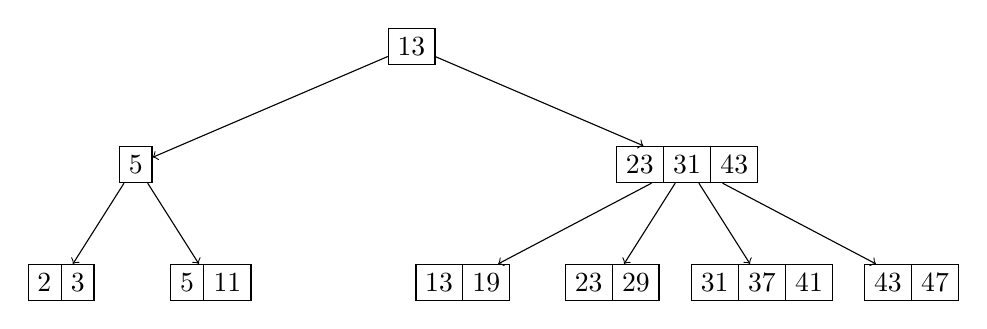
\begin{tikzpicture}
\tikzstyle{bplus}=[
  rectangle split,
  rectangle split horizontal,
  rectangle split ignore empty parts,
  draw ]
\tikzstyle{every node}=[bplus]
\tikzstyle{level 1}=[sibling distance=70mm]
\tikzstyle{level 2}=[sibling distance=19mm]
\node {13} [->]
  child {node {5}
    child {node {2 \nodepart{two} 3}}
    child {node {5 \nodepart{two} 11}}
  }
    child {node {23 \nodepart{two} 31 \nodepart{three} 43}
    child {node {13 \nodepart{three} 19}}
    child {node {23 \nodepart{two} 29}}
    child {node {31 \nodepart{two} 37 \nodepart{three} 41}}
    child {node {43 \nodepart{two} 47}}
  }
;
\end{tikzpicture}
\end{center}

\vskip.10in
\noindent After deleting 43:

\begin{center}
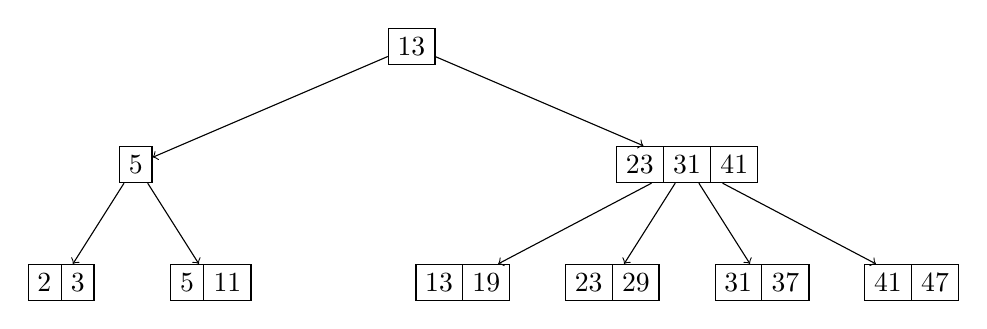
\begin{tikzpicture}
\tikzstyle{bplus}=[
  rectangle split,
  rectangle split horizontal,
  rectangle split ignore empty parts,
  draw ]
\tikzstyle{every node}=[bplus]
\tikzstyle{level 1}=[sibling distance=70mm]
\tikzstyle{level 2}=[sibling distance=19mm]
\node {13} [->]
  child {node {5}
    child {node {2 \nodepart{two} 3}}
    child {node {5 \nodepart{two} 11}}
  }
    child {node {23 \nodepart{two} 31 \nodepart{three} 41}
    child {node {13 \nodepart{three} 19}}
    child {node {23 \nodepart{two} 29}}
    child {node {31 \nodepart{two} 37}}
    child {node {41 \nodepart{two} 47}}
  }
;
\end{tikzpicture}
\end{center}

\newpage

\noindent After inserting 51:

\begin{center}
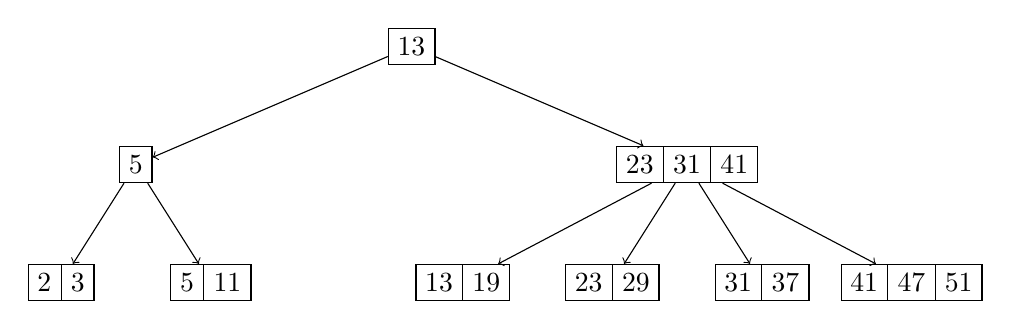
\begin{tikzpicture}
\tikzstyle{bplus}=[
  rectangle split,
  rectangle split horizontal,
  rectangle split ignore empty parts,
  draw ]
\tikzstyle{every node}=[bplus]
\tikzstyle{level 1}=[sibling distance=70mm]
\tikzstyle{level 2}=[sibling distance=19mm]
\node {13} [->]
  child {node {5}
    child {node {2 \nodepart{two} 3}}
    child {node {5 \nodepart{two} 11}}
  }
    child {node {23 \nodepart{two} 31 \nodepart{three} 41}
    child {node {13 \nodepart{three} 19}}
    child {node {23 \nodepart{two} 29}}
    child {node {31 \nodepart{two} 37}}
    child {node {41 \nodepart{two} 47 \nodepart{three} 51}}
  }
;
\end{tikzpicture}
\end{center}

\vskip.10in
\noindent After inserting 32:

\begin{center}
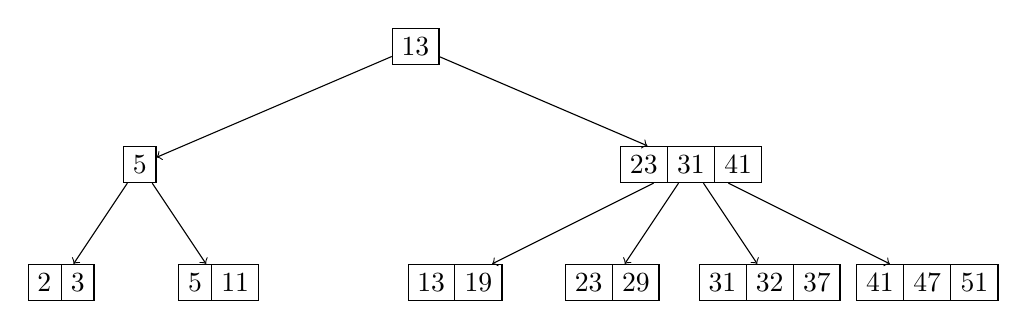
\begin{tikzpicture}
\tikzstyle{bplus}=[
  rectangle split,
  rectangle split horizontal,
  rectangle split ignore empty parts,
  draw ]
\tikzstyle{every node}=[bplus]
\tikzstyle{level 1}=[sibling distance=70mm]
\tikzstyle{level 2}=[sibling distance=20mm]
\node {13} [->]
  child {node {5}
    child {node {2 \nodepart{two} 3}}
    child {node {5 \nodepart{two} 11}}
  }
    child {node {23 \nodepart{two} 31 \nodepart{three} 41}
    child {node {13 \nodepart{three} 19}}
    child {node {23 \nodepart{two} 29}}
    child {node {31 \nodepart{two} 32 \nodepart{three} 37}}
    child {node {41 \nodepart{two} 47 \nodepart{three} 51}}
  }
;
\end{tikzpicture}
\end{center}

\vskip.35in
\noindent{\textbf{Section 5: Essay [10 points]}}

\vskip.10in
\noindent $i.$ What are the benefits to having shared locks? \\

\noindent {\textbf{Answer:}} Having shared locks means having more transactions can read the same database object. Think of the database as a blackboard and there is a teacher (a transaction) who writes to the blackboard. Also, there are students (another type of transaction) who read from the blackboard. In this example, if students are reading the blackboard (shared locks), the teacher doesn't write.

\vskip.10in
\noindent $ii.$ What does a scheduler do and what is scheduling latency? \\

\noindent {\textbf{Answer:}} Think of a scheduler as an air-traffic controller. The scheduler is responsible for coordinating concurrent transactions, giving them permission to read or write database objects. Scheduling latency refers to the time it takes before a read or write action is performed after it has been scheduled.

\vskip.10in
\noindent $iii.$ What is throughput and what are ways to increase it? \\

\noindent {\textbf{Answer:}} Throughput is the number of read or write requests performed per unit time. One way to increase throughput is to spread the data and queries across multiple disks.

\vskip.10in
\noindent $iv.$ What are different ways for disks to fail? \\

\noindent {\textbf{Answer:}} (1) Intermittent failure, (2) media failure, (3) write failure, and (4) permanent disk crash.

\vskip.10in
\noindent $v.$ What are the usual tradeoffs to consider when normalizing relations?

\noindent {\textbf{Answer:}} When normalizing, the database designer needs to consider the complexity of the resulting SQL query that would need to be written to access a normalized database. A rule of thumb when normalizing is determining if the tables are read or write intensive. Perhaps it is reasonable to store duplicate columns, if it would make the queries much more simpler.

\begin{center}
\vspace{3cm}
\textit{\lastwords}
\end{center}

\label{finalpage}

\end{document}
